\documentclass{beamer}

\usepackage{cmap}					
\usepackage{mathtext} 				
\usepackage[T2A]{fontenc}			
\usepackage[utf8]{inputenc}			
\usepackage[english,russian]{babel}
\setbeamertemplate{footline}[page number]
\setbeamertemplate{navigation symbols}{}

\title{Нечеткая кластеризация потоков данных методом d-FuzzyStream}
\institute{Высшая школа экономики}
\author{Поздняков Виталий}
\date{Декабрь 2019}

\begin{document}

\maketitle

\begin{frame}
    \frametitle{Методология FOOF (Fuzzy Online-Offline Framework)}
    \begin{itemize}
        \item Используется для работы с потоком данных
        \item Нечеткая версия OOF (Online-Offline Framework)
        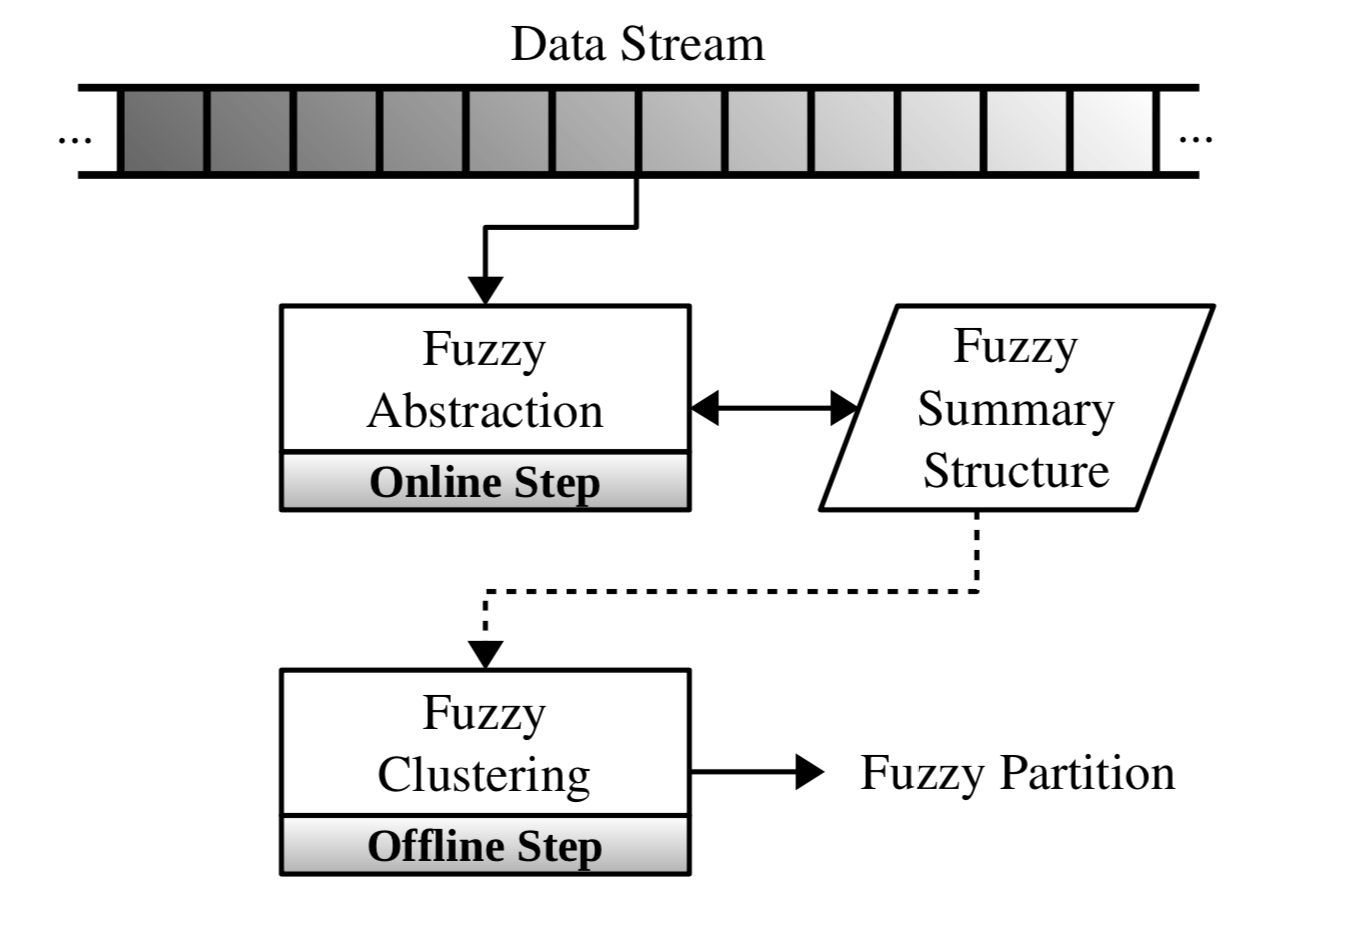
\includegraphics[width=9cm]{2019-12-18_15-01-09.png}
        \item Первый этап --- микрокластезация (d-FuzzyStreram)
        \item Второй этап --- макрокластеризация (Weighted Fuzzy C-Means)
    \end{itemize}
\end{frame}

\begin{frame}
    \frametitle{Определения}
    
    Нечеткий микрокластер (Fuzzy Micro-Claster, FMiC)  задается вектором
    $$FMiC = (\overline{CF}, SSD, N, t, M)$$
    \begin{itemize}
        \item $\overline{CF}_i = \sum \mu_{ij} x_j$ --- линейная взвешенная сумма наблюдений
        \item $SSD_i = \sum \mu_{ij}^m d(x_j, c_i)^2$ --- квадратичная взвешенная сумма расстояний до наблюдений
        \item $N_i$ --- количество наблюдений
        \item $t_i$ --- дата последнего наблюдения
        \item $M_i = \sum_{x_j \in C_i} \mu_{ij}$ --- сумма степеней принадлежности
    \end{itemize}
    Важные свойства: \textbf{инкрементность}, \textbf{аддитивность}
    
\end{frame}

\begin{frame}
    \frametitle{Определения}
    
    Тогда можно выразить
    \begin{itemize}
        \item $c = \overline{CF}/M$ --- центроид микрокластера
        \item $dp = \sqrt \frac{SSD}{N}$ --- нечеткое рассеивание (fuzzy dispersion), отражает радиус микрокластера
        \item $FR_{ij} = \frac{dp_i + dp_j}{d(c_i, c_j)}$ --- матрица близости микрокластеров $i$ и $j$. Чем больше значение, тем ближе микрокластеры
        \item  $\tau \in [0, +\infty]$ --- пороговое значение близости, при котором кластеры $i$ и $j$ объединяются в один. При $\tau < 1$ границы кластеров не пересекаются
    \end{itemize}
    
\end{frame}

\begin{frame}
    \frametitle{Алгоритм d-FuzzyStream}
    
    Входные параметры:
    $minFMiC$, $maxFMiC$ --- минимальное и максимальное количество микрокластеров, $\tau$ --- порог объединения микрокластеров, $m$ --- коэффициент размытия
    
    \begin{enumerate}
        \item Пока количество микрокластеров меньше минимального, создаем новые микрокластеры под каждое наблюдение
        \item Если новое наблюдение попадает в радиус хотя бы одного микрокластера, то оно инкрементируется в параметры этих микрокластеров со степенью принадлежности
        $$\mu_{ik} = 1 / \sum_j \left( \frac{d(x_k, v_i)^2}{d(x_k, v_j)^2} \right)^{\frac{1}{m-1}}$$
        \item Если новое наблюдение не попадает в радиус микрокластера, то создаем под него новый микрокластер
        \item При превышении максимального количества кластеров удаляется самый старый
        \item При превышении порога близости кластеры объединяются
    \end{enumerate}
    
\end{frame}

\begin{frame}
    \centering
    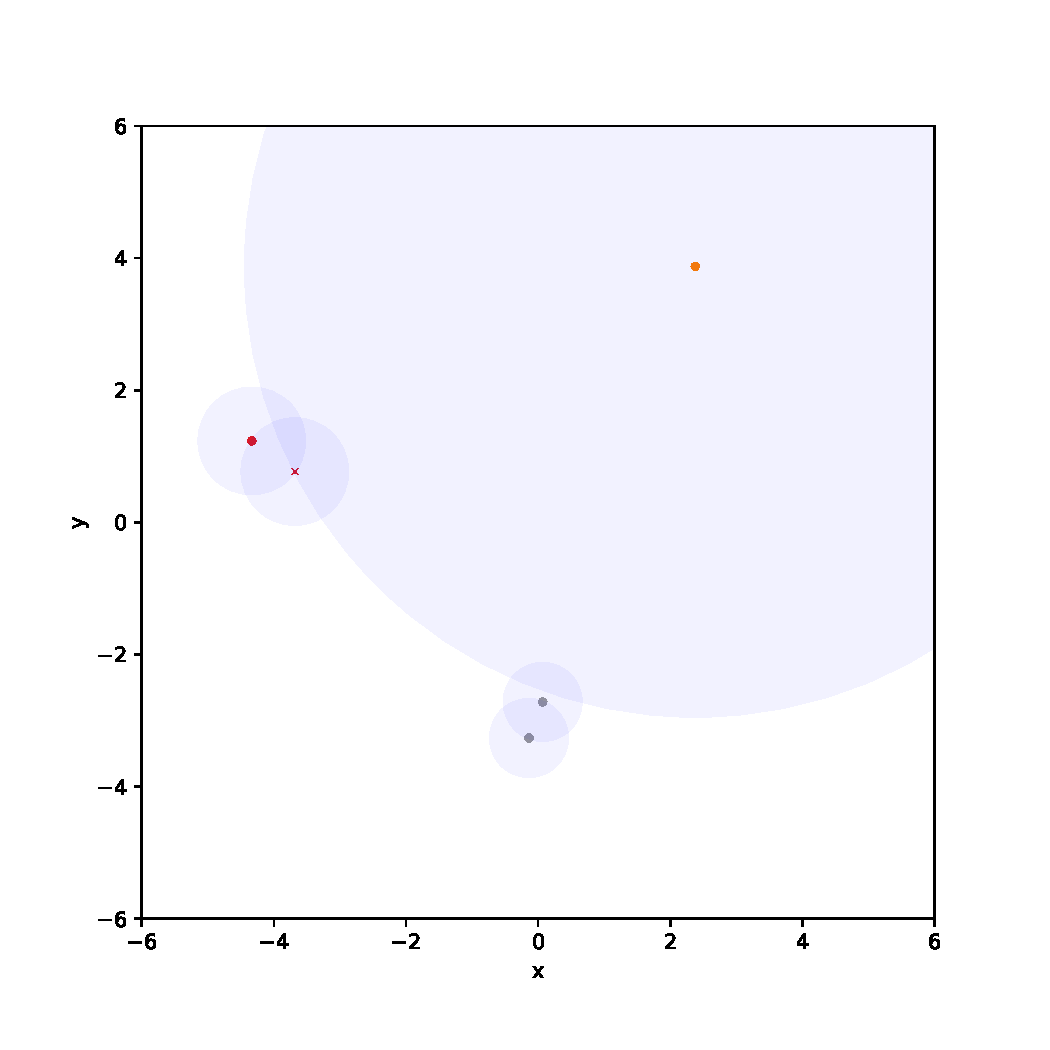
\includegraphics[width=9.1cm]{step1.pdf}
\end{frame}

\begin{frame}
    \centering
    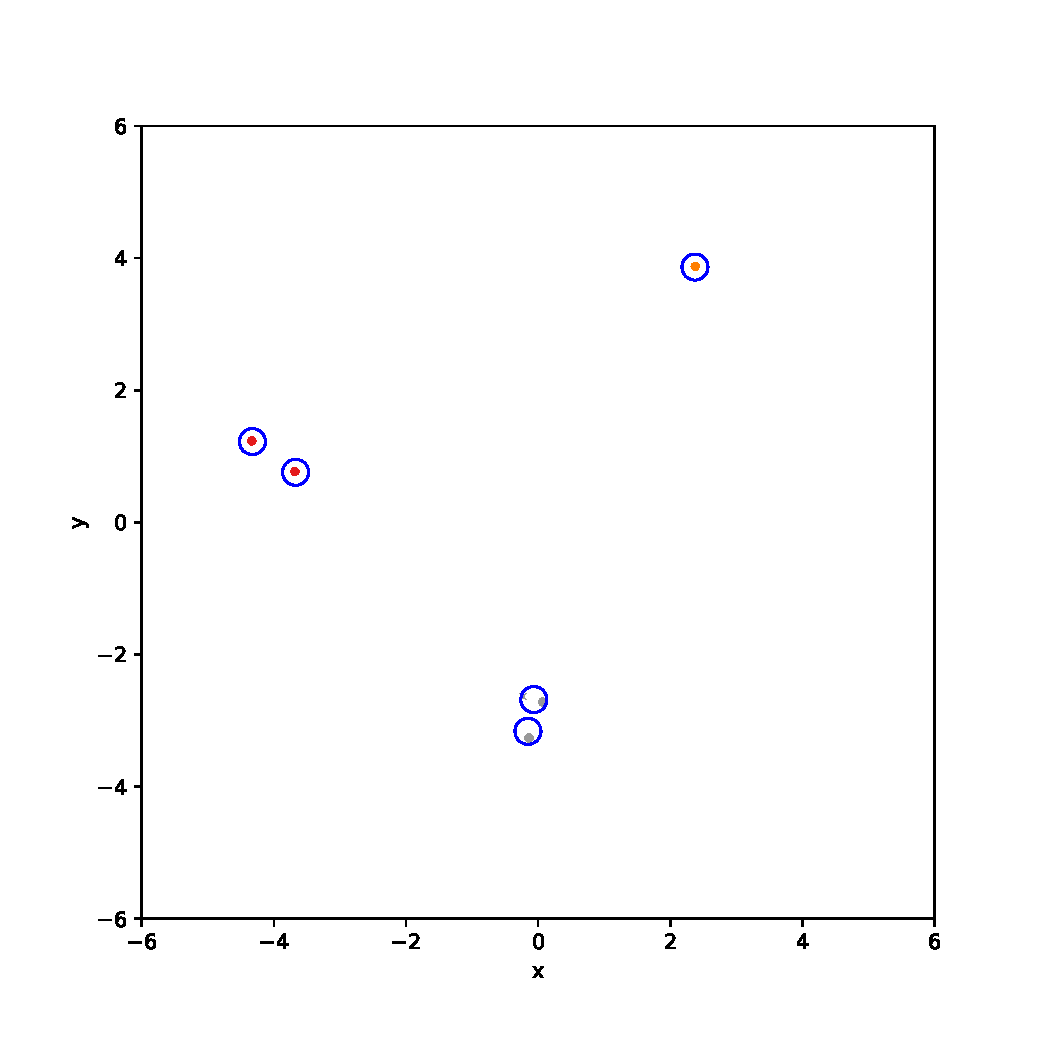
\includegraphics[width=9.1cm]{step2.pdf}
\end{frame}

\begin{frame}
    \centering
    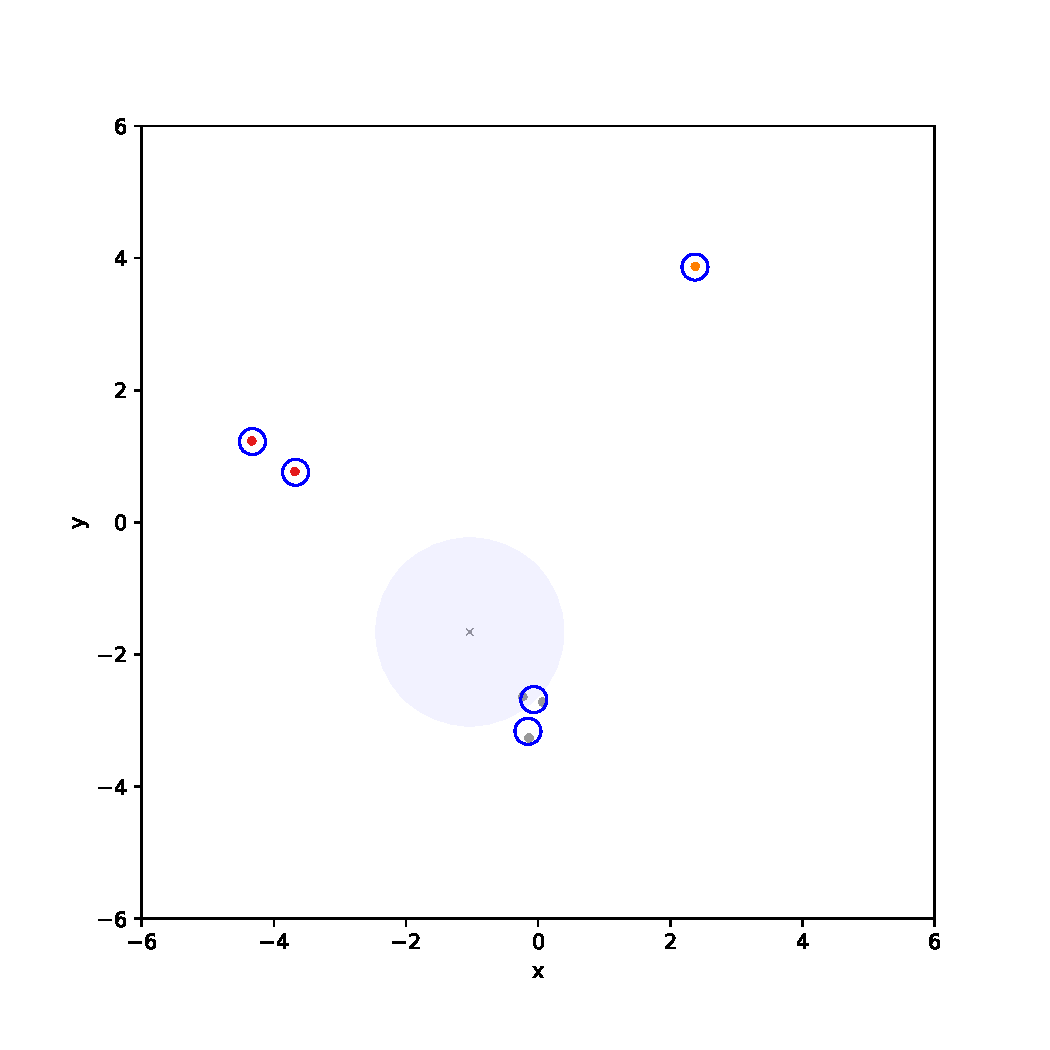
\includegraphics[width=9.1cm]{step3.pdf}
\end{frame}

\begin{frame}
    \centering
    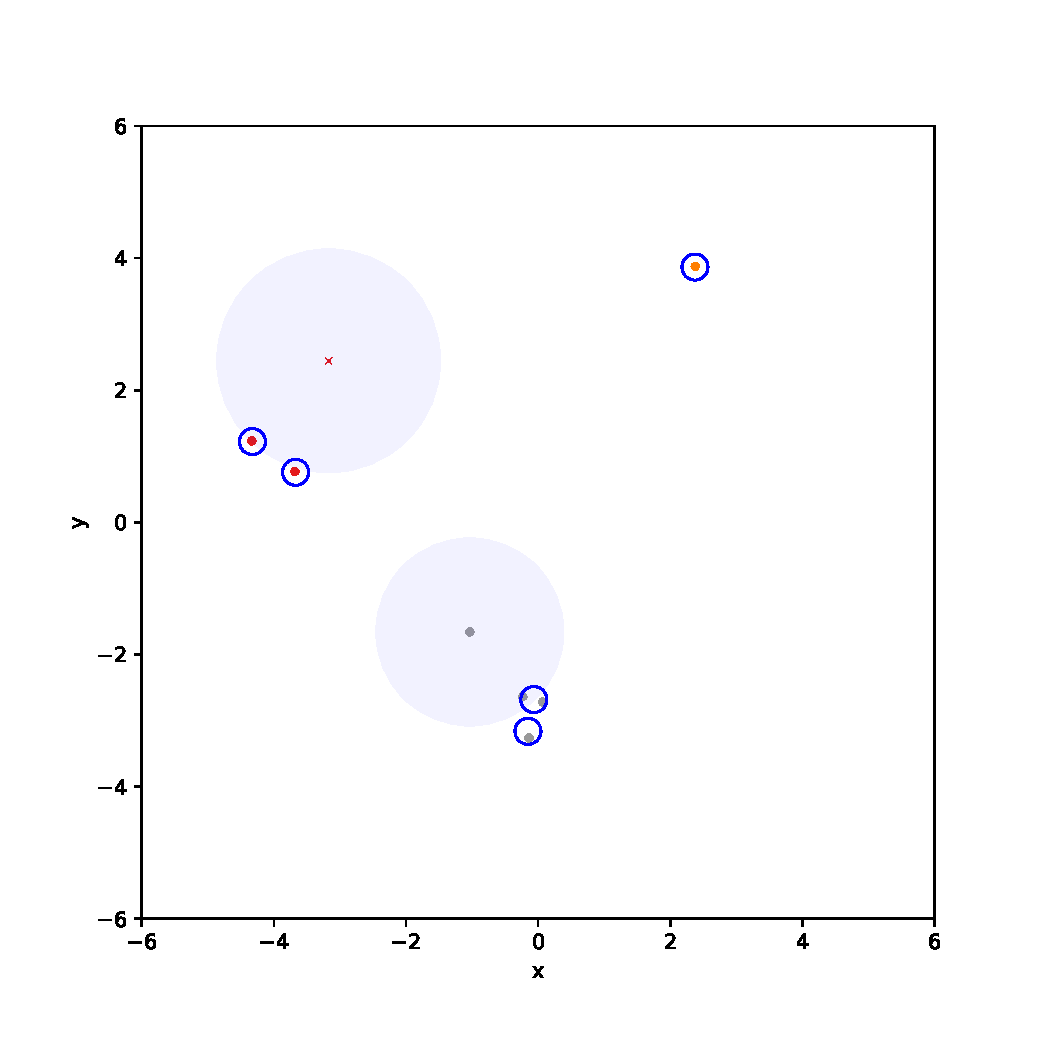
\includegraphics[width=9.1cm]{step4.pdf}
\end{frame}

\begin{frame}
    \centering
    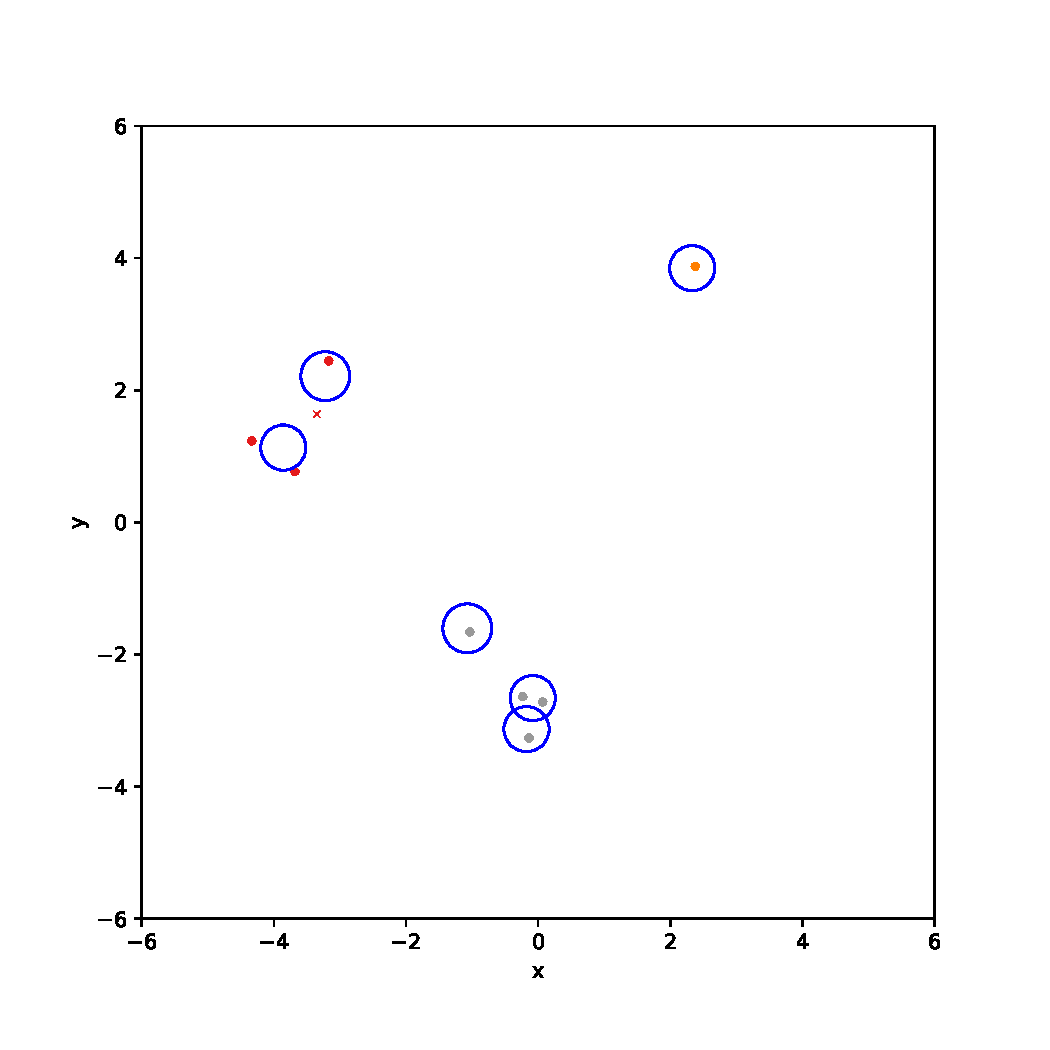
\includegraphics[width=9.1cm]{step5.pdf}
\end{frame}

\begin{frame}
    \centering
    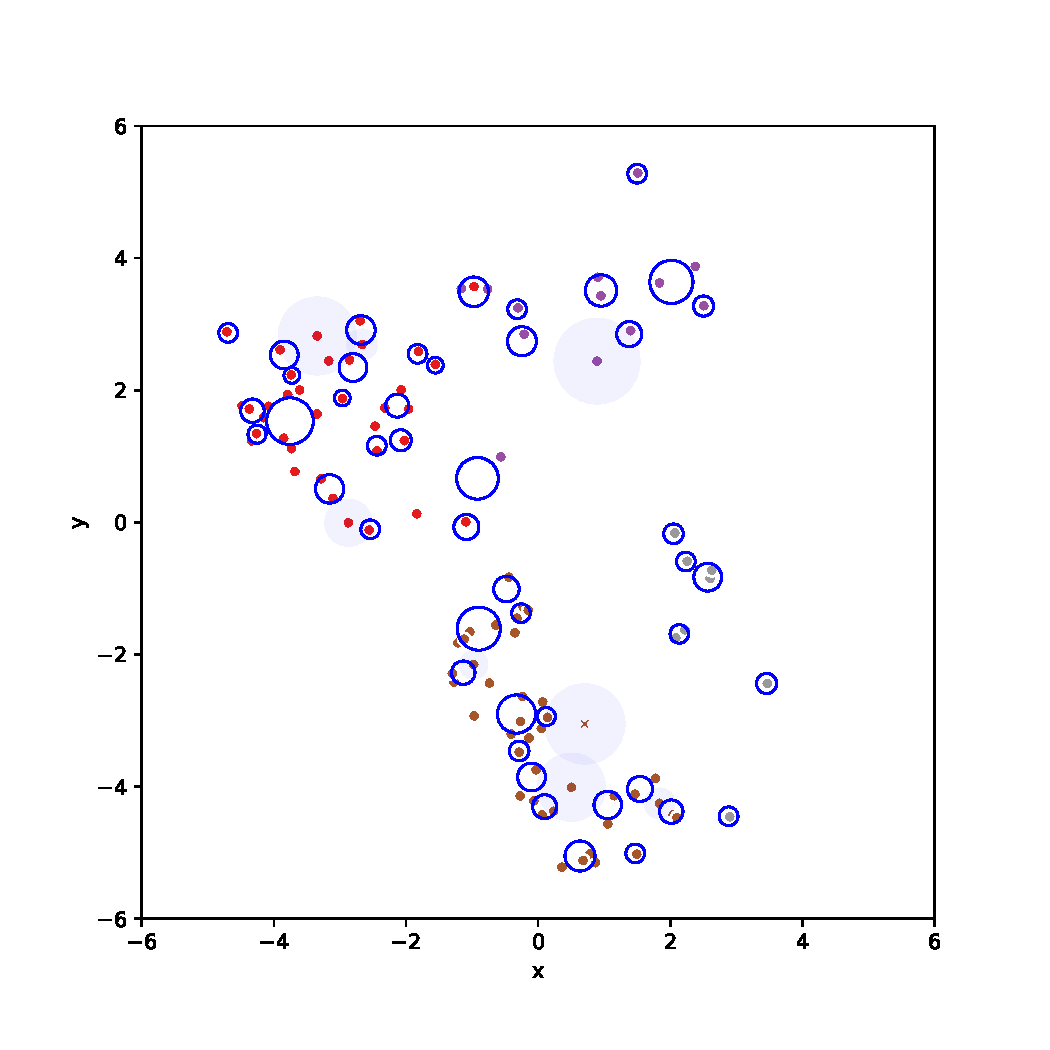
\includegraphics[width=9.1cm]{step6.pdf}
\end{frame}

\begin{frame}
    \frametitle{Датасеты для тестирования}
    
    \begin{itemize}
        \item Сгенерированные 10000 наблюдений (3 временных среза)
        
        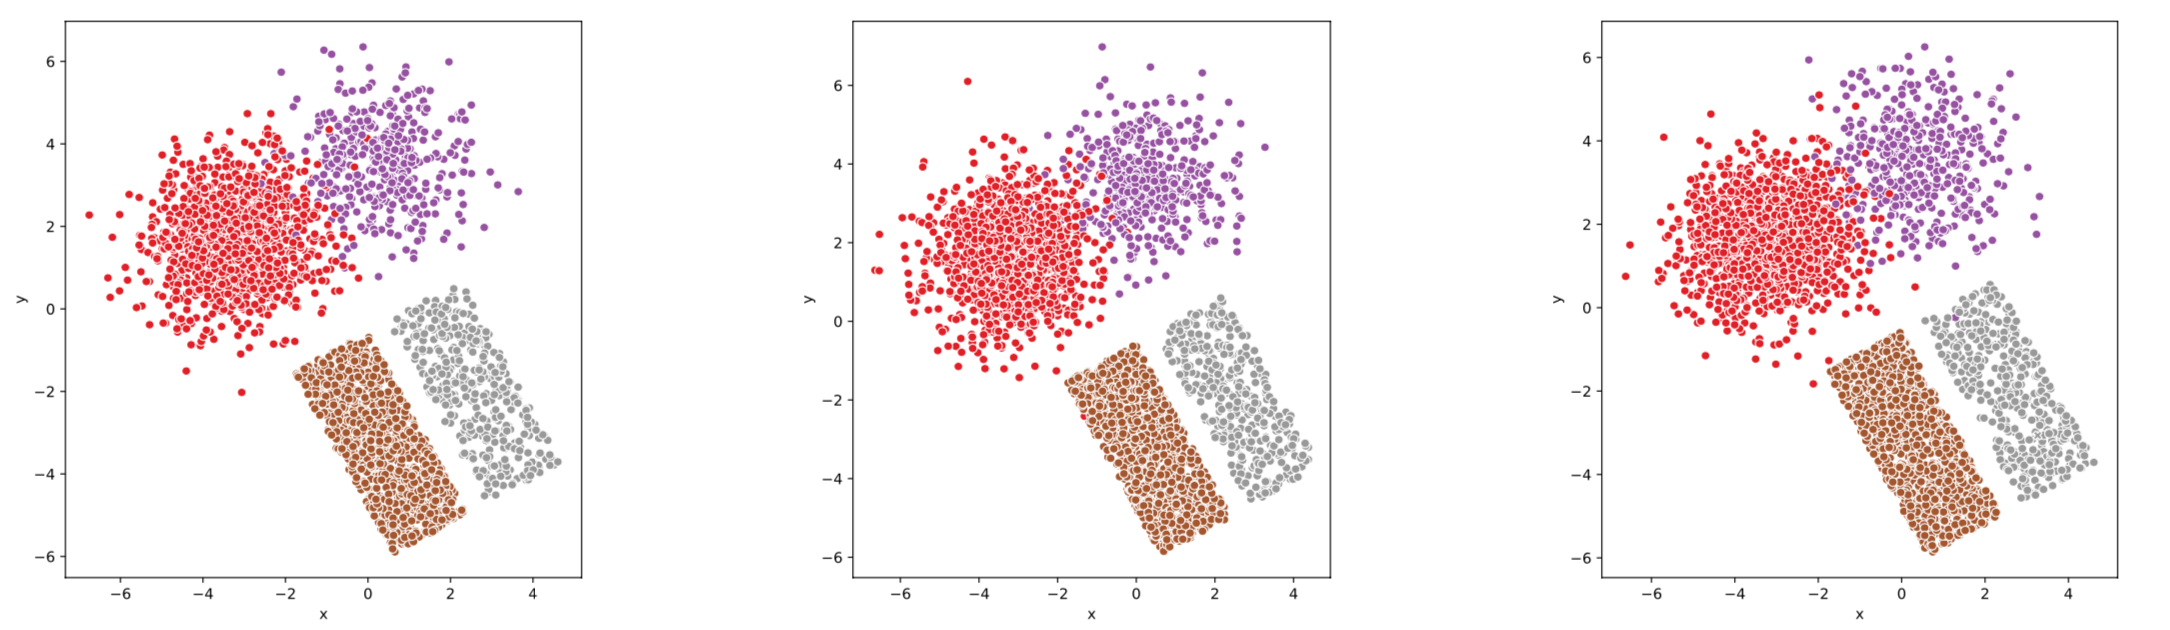
\includegraphics[width=10cm]{2020-01-29_03-29-26.png}
        
        \item Сгенерированные 11000 наблюдений (3 временных среза)
        
        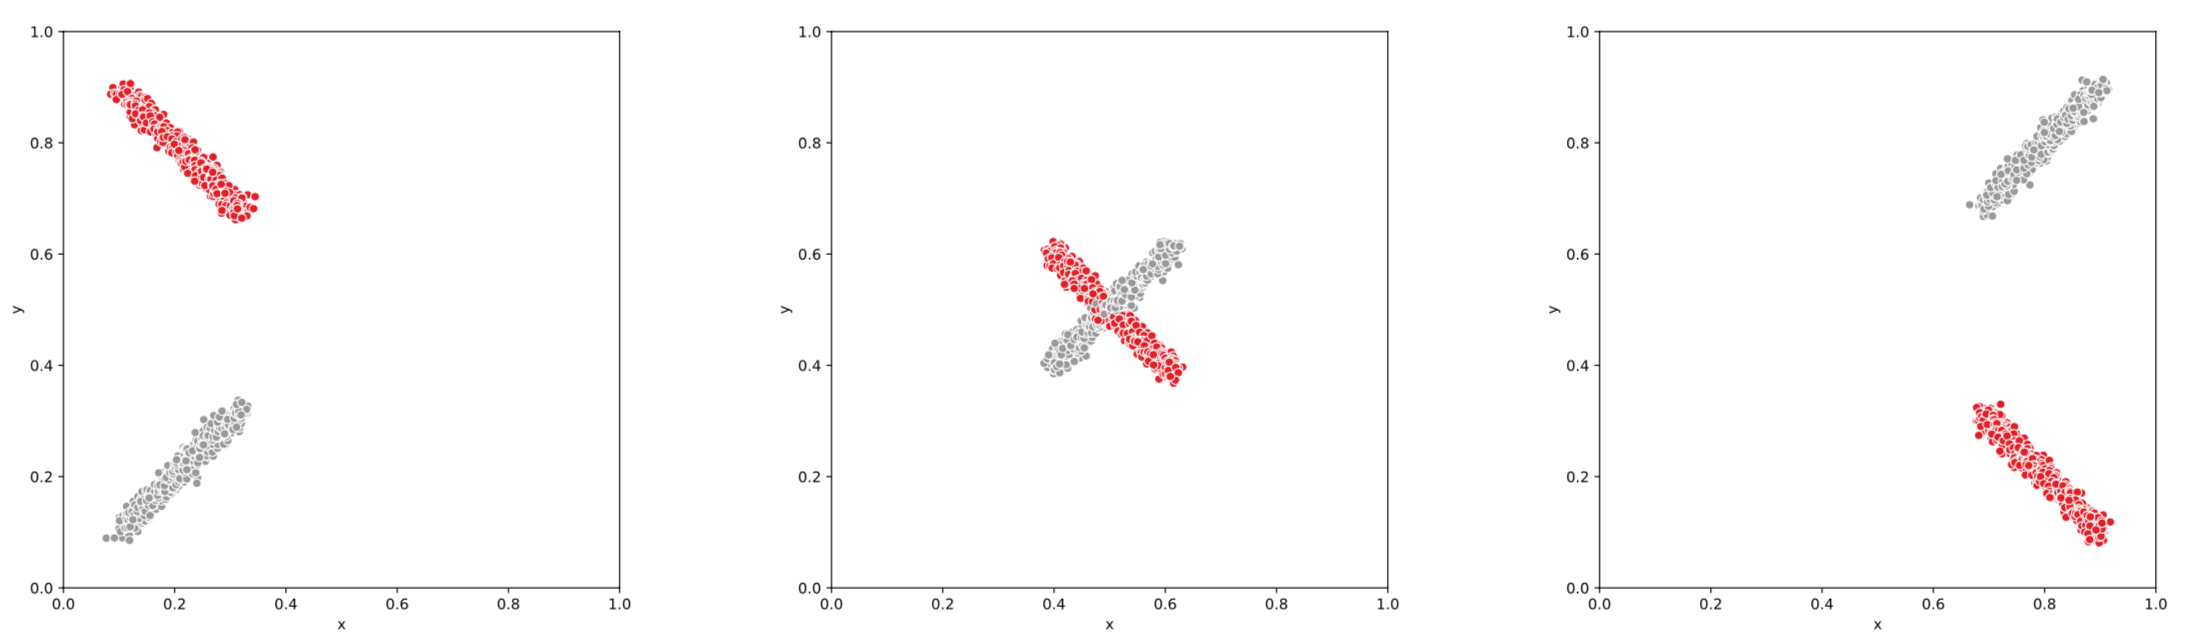
\includegraphics[width=10cm]{2020-01-29_03-29-44.png}
        
    \end{itemize}

\end{frame}

\begin{frame}{Метрики качества}

    \begin{itemize}
        \item $Creations$ --- количество созданных микрокластеров
        \item $Removals$ --- количество удаленных микрокластеров
        \item $Absorptions$ --- количество попаданий в радиус микрокластера
        \item $Merges$ --- количество объединений микрокластеров
        \item $Purity = \frac{1}{N} \sum_i \max_j \vert C_i \cap T_j \vert$ --- мера <<чистоты>> кластеризации, где $T_j$ --- размеченный заранее класс наблюдения
    \end{itemize}
    
\end{frame}

\begin{frame}{Результаты тестирования}
\centering
    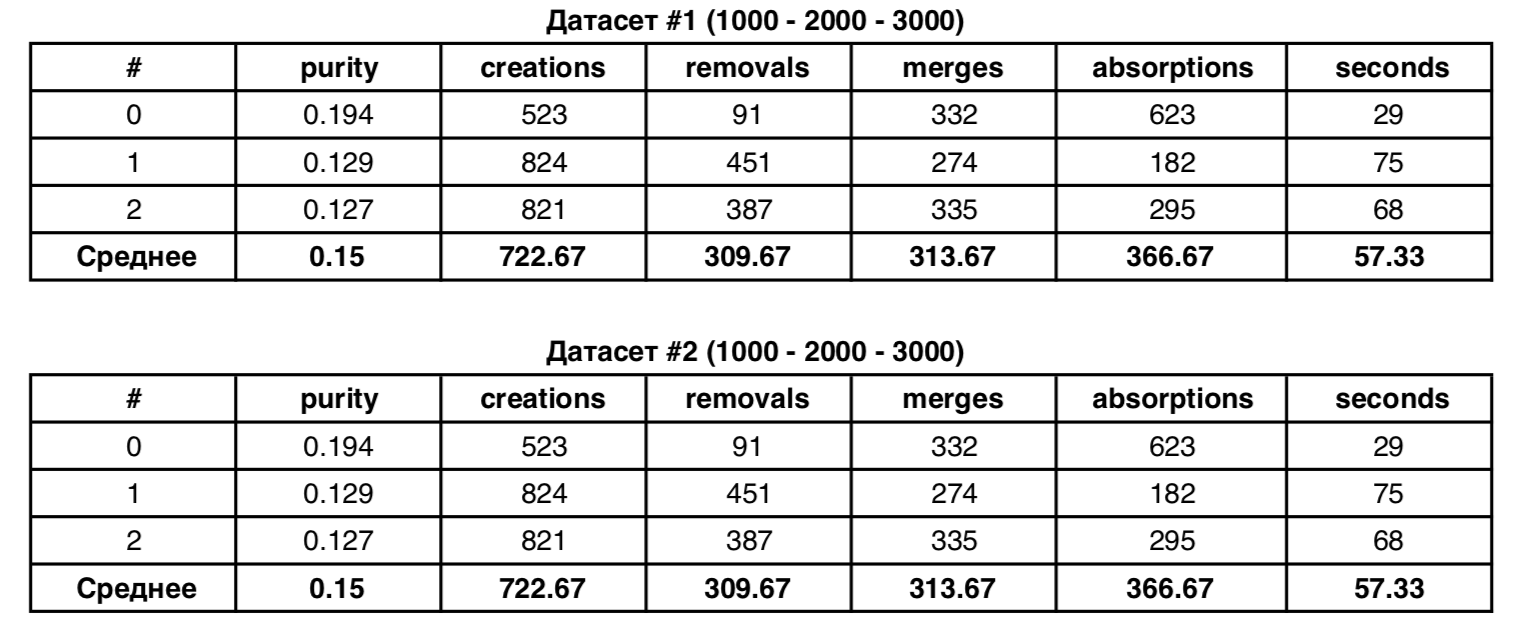
\includegraphics[width=\textwidth]{2019-12-20_16-54-26.png}
\end{frame}

\begin{frame}
    \frametitle{Литература}
    
    \begin{itemize}
        \item A Framework for Clustering Evolving Data Streams, 2003, Charu C. Aggarwal, Jiawei Han, Jianyong Wang, Philip S. Yu
        \item FuzzStream: Fuzzy Data Stream Clustering Based on the Online-Offline Framework, 2017, Priscilla de Abreu Lopes and Heloisa de Arruda Camargo
        \item d-FuzzStream: A Dispersion-Based Fuzzy Data Stream Clustering, 2018, Leonardo Schick, Priscilla de Abreu Lopes and Heloisa de Arruda Camargo
        \item Merging Clusters in Summary Structures for Data Stream Mining based on Fuzzy Similarity Measures, 2019, Leonardo Schick, Priscilla de Abreu Lopes and Heloisa A. Camargo
    \end{itemize}
    
\end{frame}

\end{document}
